\chapter{Control Vehículo}

\thispagestyle{plain}
\renewcommand{\tablename}{Tabla}

\section{Introducción}

En este capítulo se desarrollarán todos los subsistemas y modelos dedicados al control del vehículo robótico a través de la placa Arduino. 

\section{Subsistemas Simulink}

\subsection{\textit{Receive from PC}}

Este primer subsistema es el encargado de recibir la consigna de velocidad linear y angular, además del modo de funcionamiento desde el ordenador. El bloque `\textit{Serial Receive}' se configurará de manera que los datos recibidos sean del tipo \textit{uint8} y con un tamaño de 20, esto viene determinado del `\textit{Serial Send}' del ordenador. A diferencia del modelo del PC en el que su \textit{Serial Receive} permitía la determinación de las características de la trama de datos además del \textit{Header} y \textit{Terminator}, en este caso estos últimos no se pueden configurar, haciendo necesario el uso del bloque `\textit{Protocol Decoder}'. Este bloque debe tener la misma configuración que el `\textit{Protocol Encoder}' del modelo del ordenador (Figura \ref{fig:Block Parameters-Protocol Encoder PC}).

\begin{figure}[H]
    \centering
    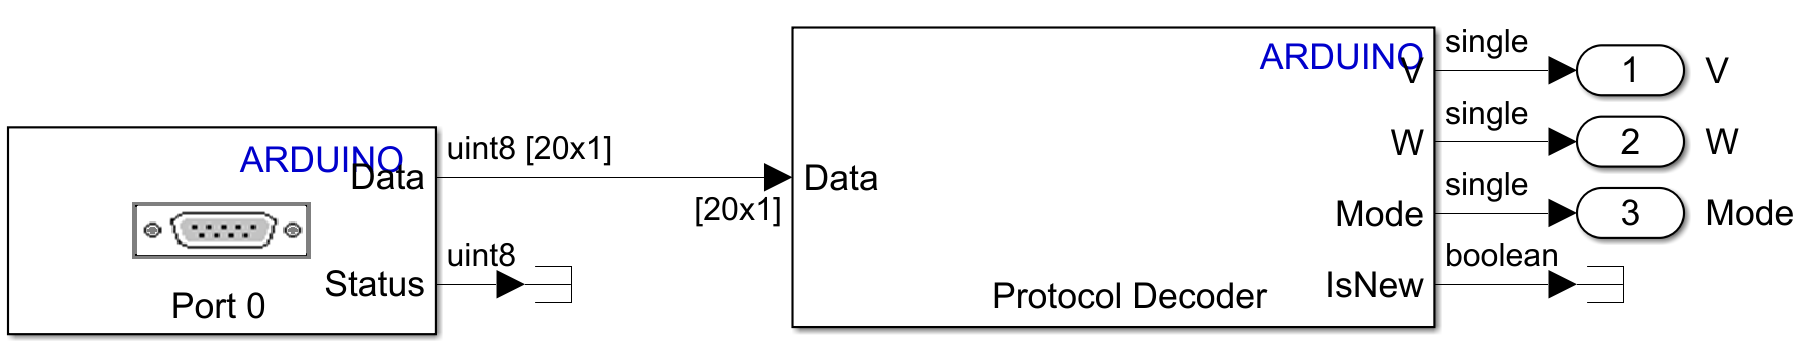
\includegraphics[width=1\linewidth]{imagenes/Simulink - Control Vehiculo - Receive from PC.png}
    \caption{Subsistema \textit{Receive from PC}}
    \label{fig:Subsistema - Receive from PC}
\end{figure}

\begin{figure}[H]
     \centering
     \begin{subfigure}[c]{0.45\textwidth}
         \centering
         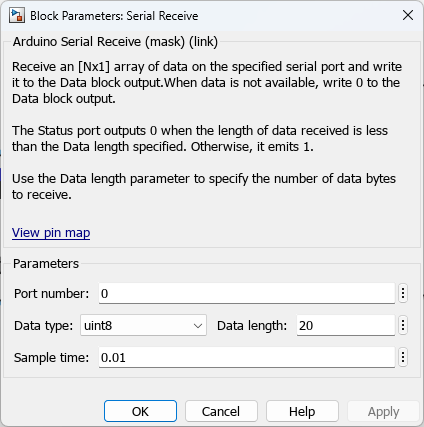
\includegraphics[width=1\textwidth]{imagenes/Simulink - Block Parameters - Serial Receive Arduino.png}
         \caption{Serial Receive}
     \end{subfigure}
     \hfill
     \begin{subfigure}[c]{0.45\textwidth}
         \centering
         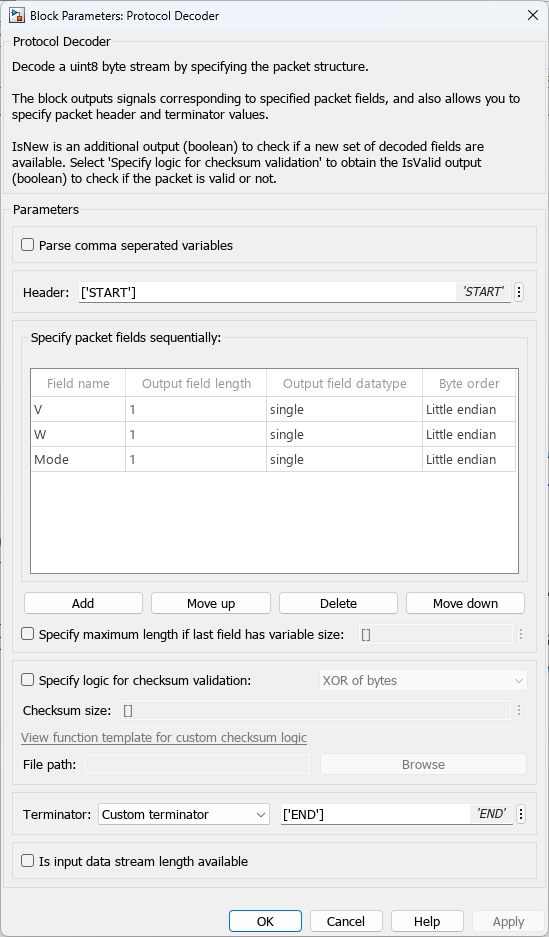
\includegraphics[width=1\textwidth]{imagenes/Simulink - Block Parameters - Protocol Decoder Arduino.png}
         \caption{Protocol Decoder}
     \end{subfigure}
        \caption{Parámetros de los bloques.}
\end{figure}

\subsection{Modelo cinemático inverso}

Este subsistema utiliza las distintas operaciones matemáticas necesarias para transformar las velocidades lineales, \(v\), y angulares, \(\omega\) del vehículo en las velocidades individuales de cada una de las seis ruedas. Para ello es necesario establecer una serie de parámetros que definan la geometría del chasis:
\begin{itemize}
    \item R: Radio de ruedas.
    \item Lx: Distancia longitudinal desde el centro del chasis hasta las ruedas delanteras y traseras.
    \item Ly: Distancia lateral desde el centro del chasis hasta las ruedas laterales
    \item b: Ancho del chasis
\end{itemize}

\begin{figure}[H]
    \centering
    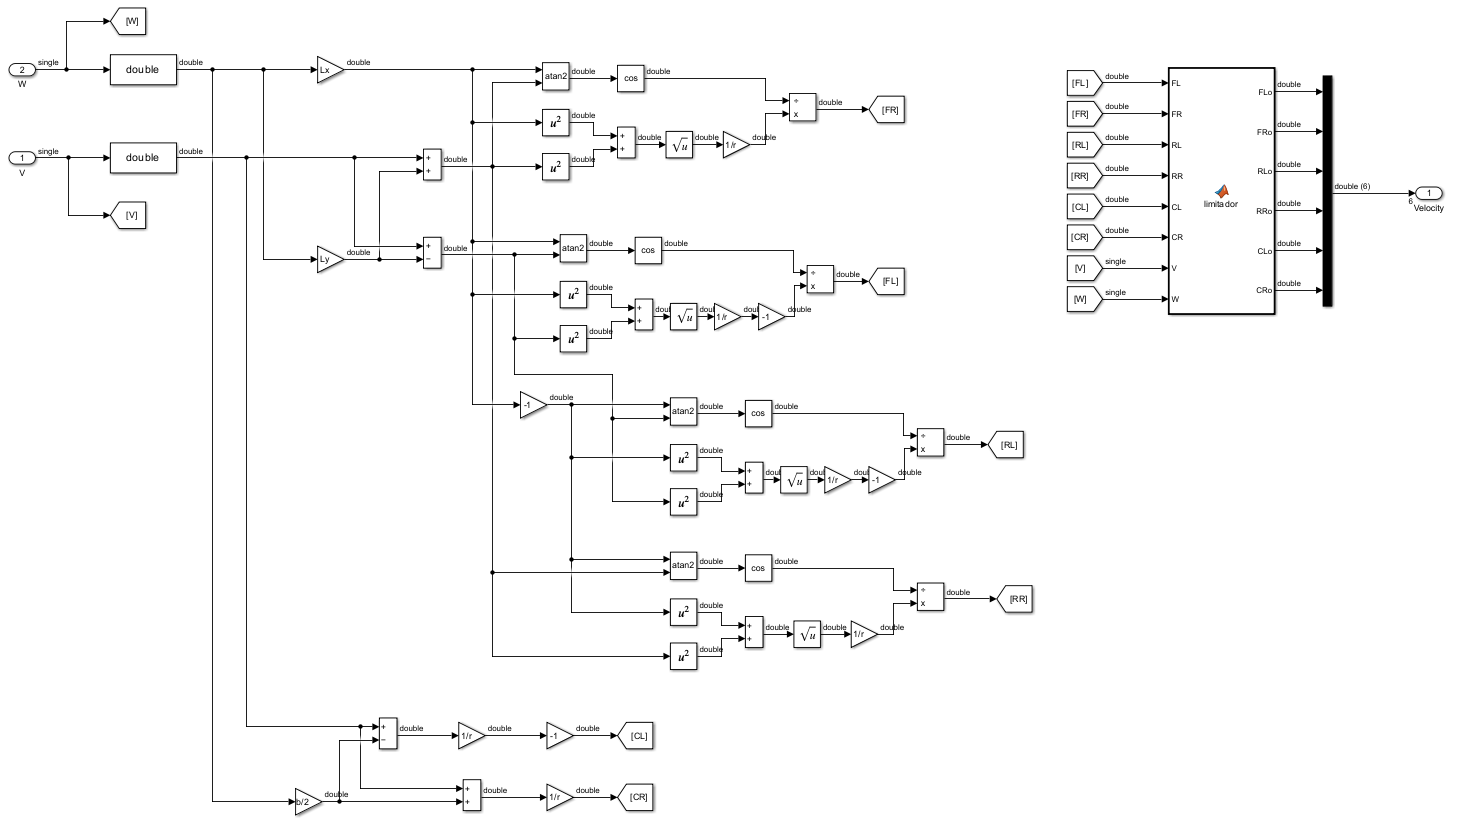
\includegraphics[width=1\linewidth]{imagenes/Simulink - Control Vehiculo - MCI.png}
    \caption{Subsistema Modelo Cinemático Inverso}
    \label{fig:Subsistema - MCI}
\end{figure}

En este mismo subsistema se añade una función de MATLAB, cuyo código `Limitador' se encuentra en el anexo \ref{MATLAB Functions}. Esta función ajusta las velocidades de las ruedas del vehículo robótico en función de las entradas de velocidad lineal y angular. Si ambas velocidades son diferentes de cero, se corrigen las velocidades de las ruedas centrales y estas velocidades ajustadas se propagan a las ruedas delanteras y traseras. Si una de las velocidades es cero, se mantienen las velocidades originales.

\subsection{Control Ruedas}

\begin{figure}[H]
    \centering
    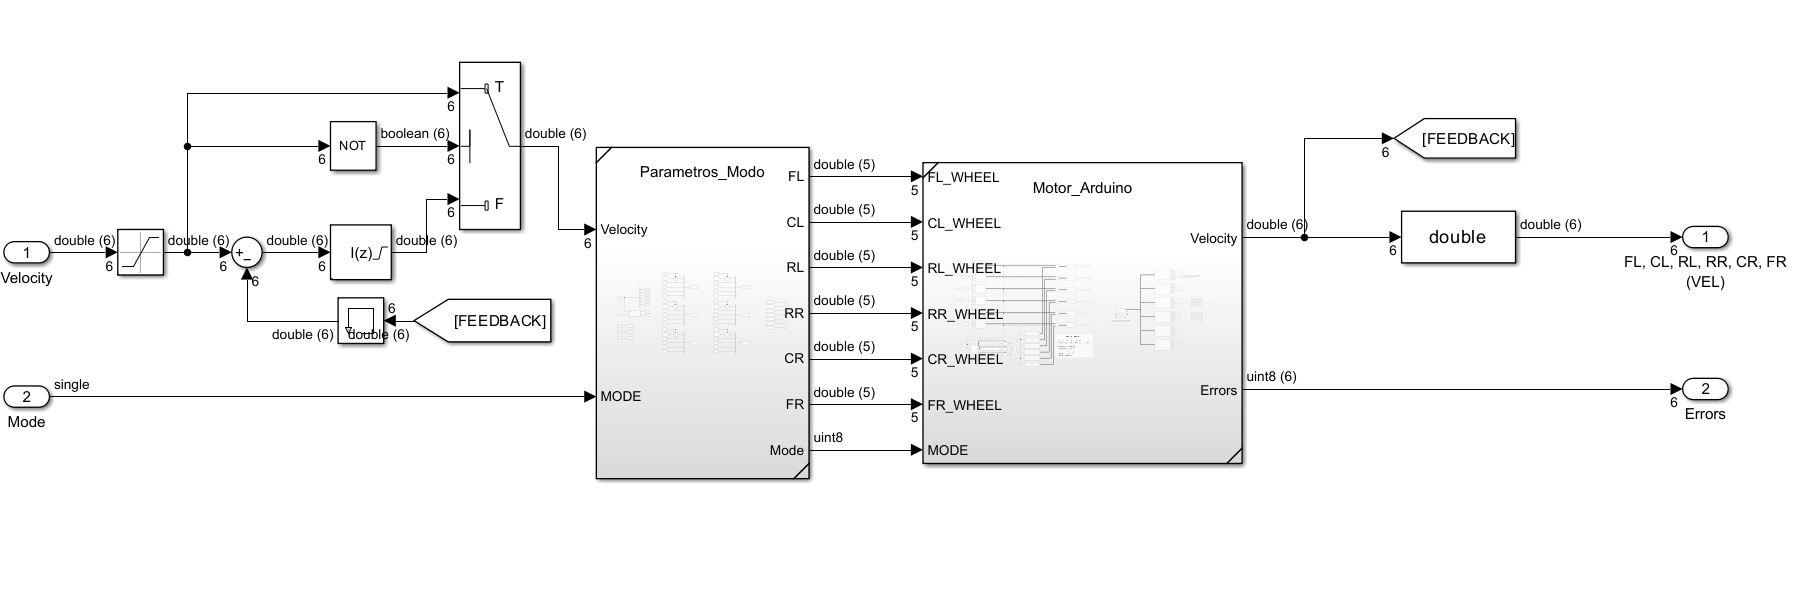
\includegraphics[width=1\linewidth]{imagenes/Simulink - Control Vehiculo - Control Ruedas.png}
    \caption{Subsistema Control Ruedas}
    \label{fig:Subsistema - Control Ruedas}
\end{figure}

\subsubsection{Parámetros Modo}

\begin{figure}[H]
    \centering
    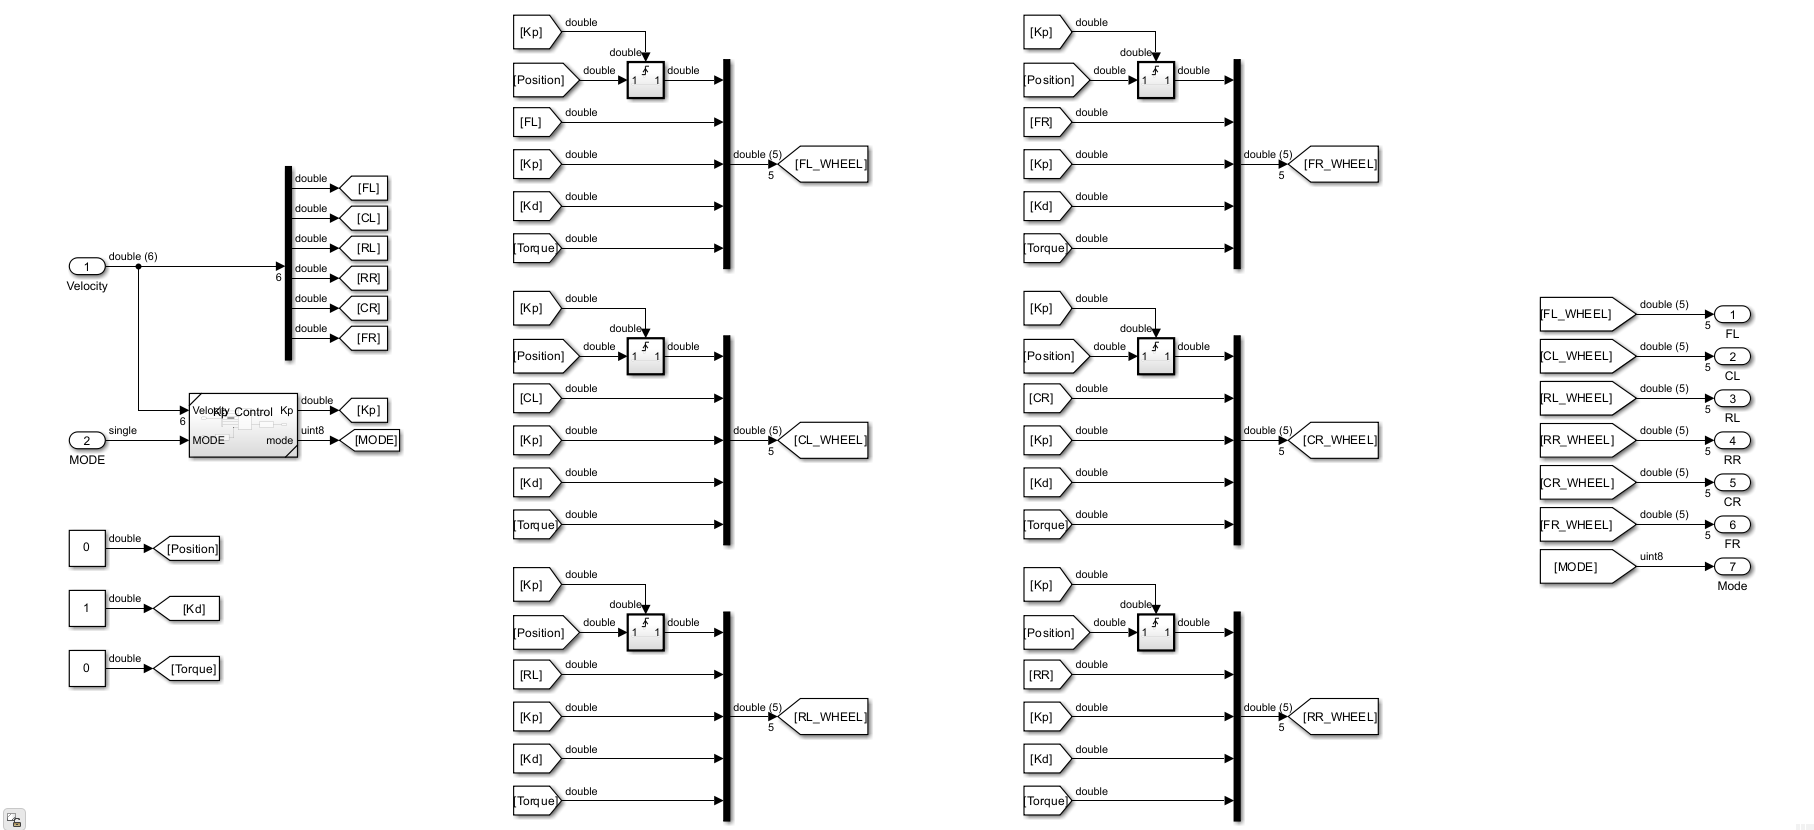
\includegraphics[width=1\linewidth]{imagenes/Simulink - Control Vehiculo - Control Ruedas - Parametros Modo.png}
    \caption{Subsistema Parámetros Modo}
    \label{fig:Subsistema - Parametros Modo}
\end{figure}

La función principal de este subsistema es crear los vectores que se utilizarán posteriormente para cada uno de los motores. Como entrada recibe el vector de seis velocidades correspondientes a cada una de las ruedas, y el modo de funcionamiento. Con esto se calcula Kp y el modo que finalmente se utilizará, haciendo uso del subsistema de control de Kp (Figura \ref{fig:Subsistema - Kp Control}). Este subsistema tendrá seis salidas que corresponderán a cada uno de los motores y contendrán el vector de parámetros de control de estos.

\begin{figure}[H]
    \centering
    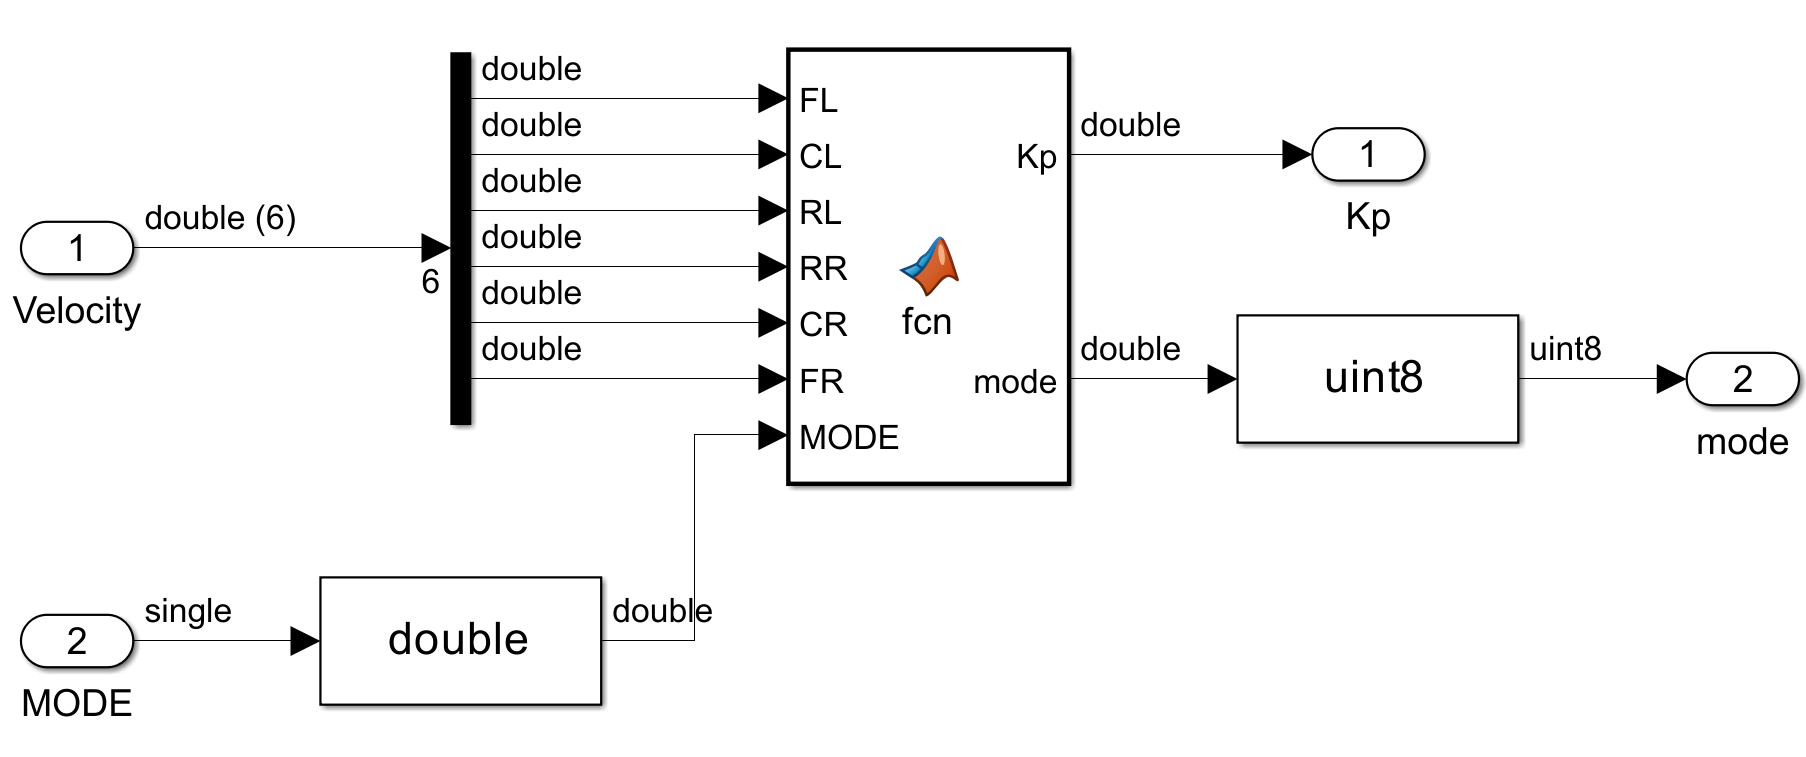
\includegraphics[width=1\linewidth]{imagenes/Simulink - Control Vehiculo - Control Ruedas - Kp Control.png}
    \caption{Subsistema Control Kp}
    \label{fig:Subsistema - Kp Control}
\end{figure}

El código del bloque `\textit{MATLAB Function}' se puede encontrar en el Apéndice \ref{MATLAB Functions}, este determinará los valores de Kp y \textit{mode} en función de las velocidades y modo de funcionamiento de entrada. En caso de que todas las velocidades sean cero y el modo sea `1', Kp tendrá un valor de 25 y \textit{mode} cambiará a `2' (control de posición). En caso contrario Kp se establece a 0 y \textit{mode} se mantiene igual a la entrada. 

\subsubsection{Motor Arduino}

Este subsistema es el encargado de comunicarse con las ruedas. Mandando las señales de control y recibiendo el estado de estos. El funcionamiento de dicho subsistema se desarrolló más en profundidad en apartados previos de la memoria. 

\begin{figure}[H]
    \centering
    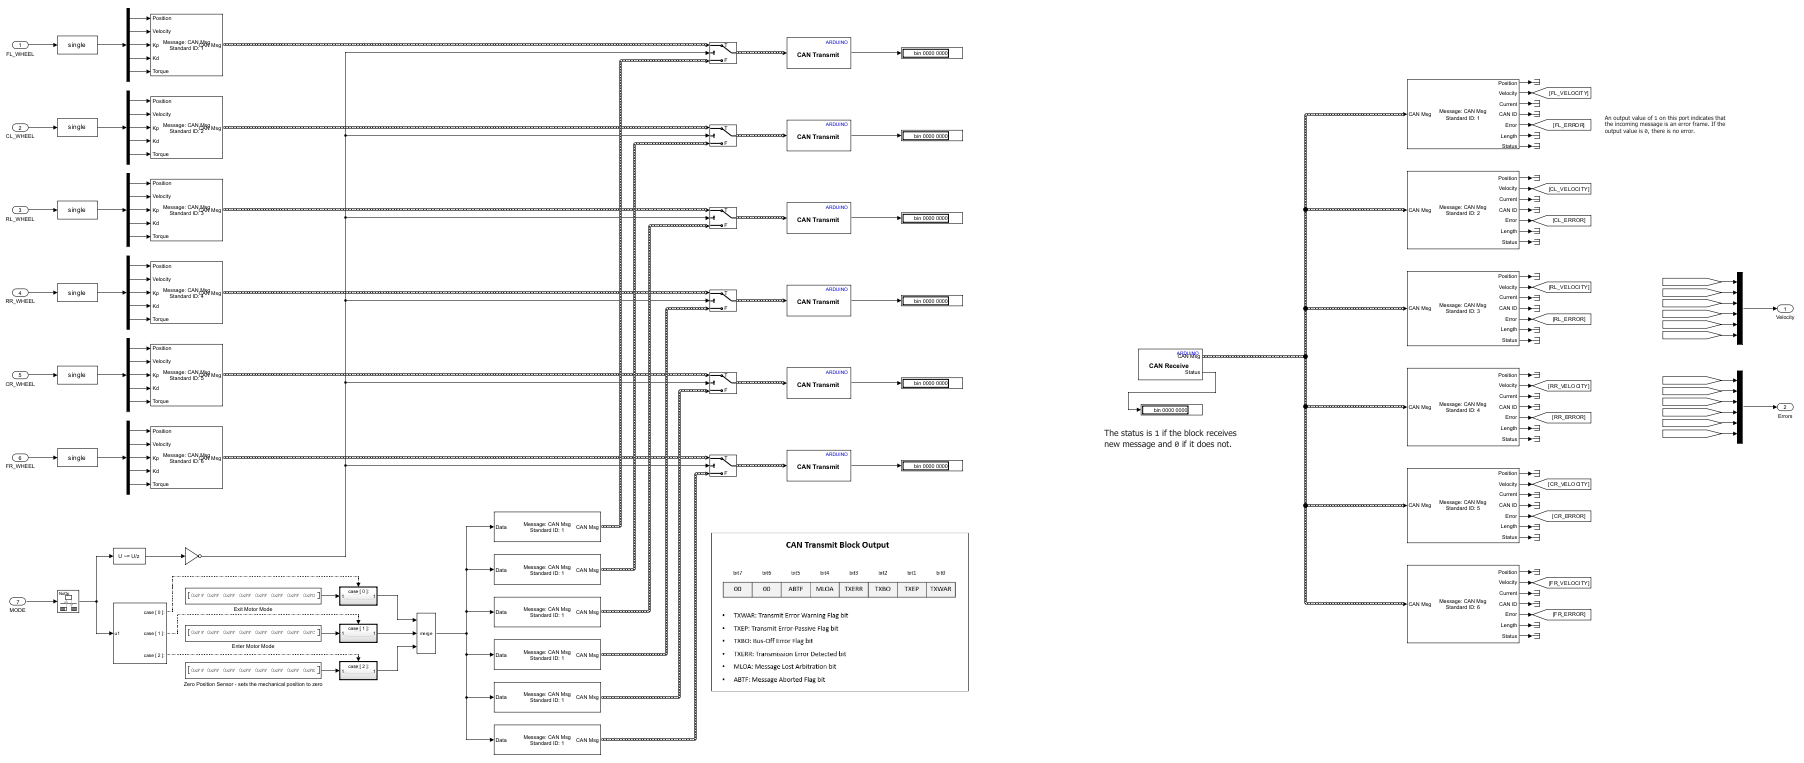
\includegraphics[width=1\linewidth]{imagenes/Simulink - Control Vehiculo - Control Ruedas - Ruedas.png}
    \caption{Subsistema Ruedas}
    \label{fig:Subsistema - Ruedas}
\end{figure}

En resumen, este subsistema tendrá siete entradas, seis de ellas correspondientes a los motores y una última de modo de funcionamiento. Las entradas perteneciente a los motores, son vectores de cinco parámetros: Posición, Velocidad, Kp, Kd y Torque. Estos serán empaquetados en un mensaje CAN y transmitidos al motor en todo momento, a excepción de los cambios de modo de funcionamiento. Por otro lado, este subsistema también recibe la información de los motores, desempaquetando esta para cada uno de los motores y sacando un vector de velocidades y otro de detección de errores.

\subsection{Modelo cinemático directo}

El modelo cinemático directo describe la relación entre las velocidades individuales de las ruedas y el movimiento global para el vehículo en términos de su velocidad lineal y angular. Se toman las ruedas centrales como motrices, sólo se utilizan las velocidades de estas para el cálculo.

\begin{figure}[H]
    \centering
    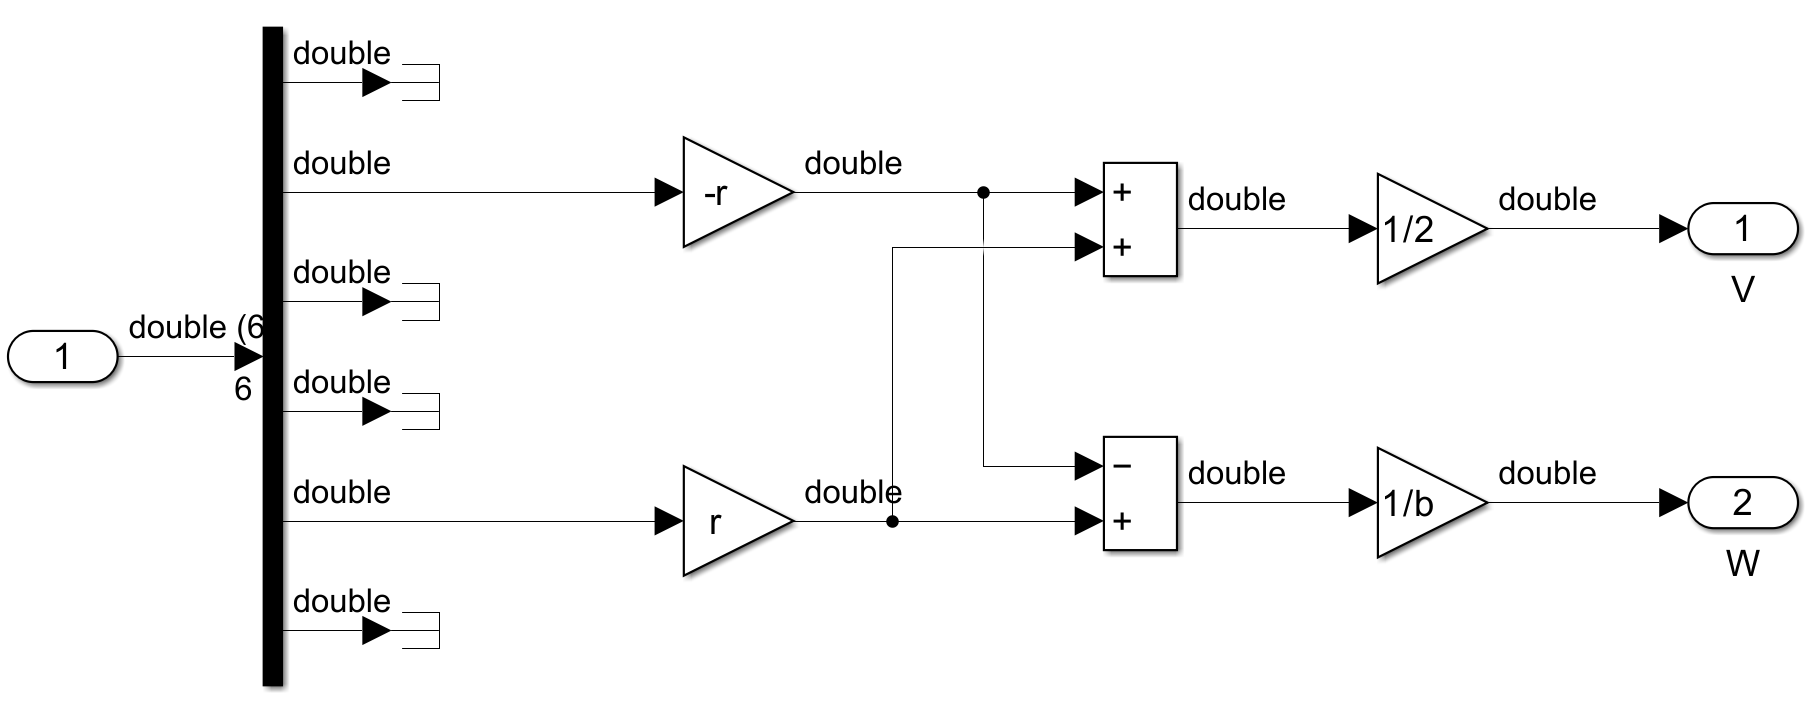
\includegraphics[width=1\linewidth]{imagenes/Simulink - Control Vehiculo - MCD.png}
    \caption{Subsistema Modelo Cinemático Directo}
    \label{fig:Subsistema - MCD}
\end{figure}

Este modelo implementa las siguientes ecuaciones:

\begin{equation}
    v = \frac{R \times (v_{CR} - v_{CL})}{2}
\end{equation}

\begin{equation}
    v = \frac{R \times (v_{CR} + v_{CL})}{b}
\end{equation}

\subsection{\textit{Send to PC}}

La finalidad de este subsistema será la de transmitir la velocidad linear y angular del vehículo al PC. La configuración del bloque `\textit{Protocol Encoder}' es hermana de la de, en este caso, el `\textit{Serial Receive}' del modelo del ordenador (Figura \ref{fig:Block Parameters - Serial Receive PC}). Con la finalidad de no saturar el puerto de comunicación de la placa Arduino, el bloque `\textit{Serial Transmit}' se incluye dentro de un \textit{Enabled Subsystem} que se activará únicamente cuando la información que se quiera transmitir haya cambiado.

\begin{figure}[H]
    \centering
    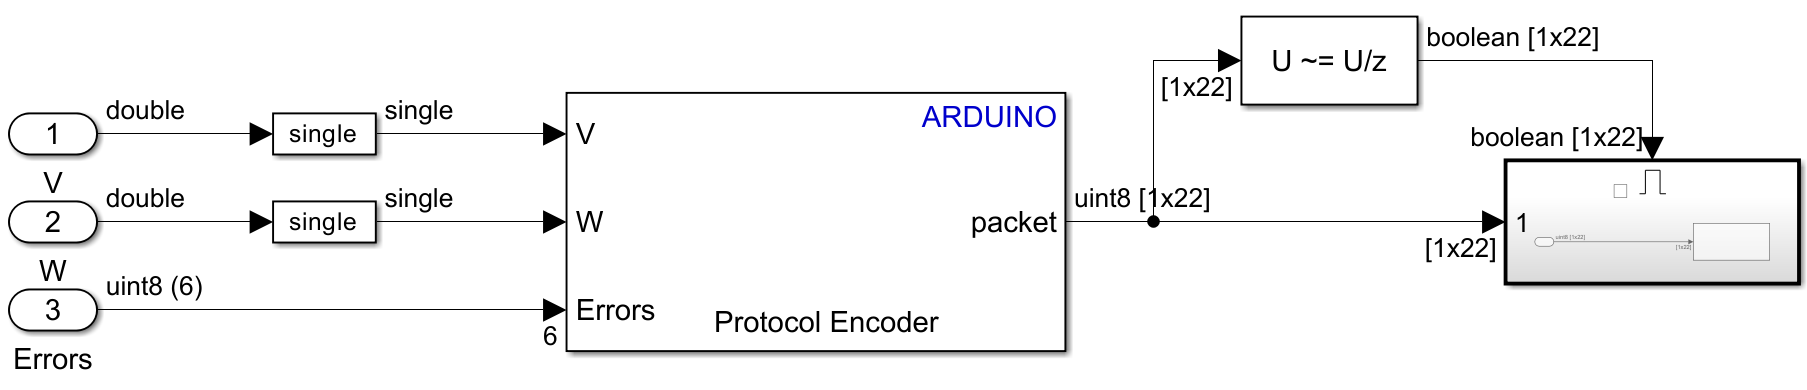
\includegraphics[width=1\linewidth]{imagenes/Simulink - Control Vehiculo - Send to PC.png}
    \caption{Subsistema Send to PC}
\end{figure}

\begin{figure}[H]
     \centering
     \begin{subfigure}[c]{0.45\textwidth}
         \centering
         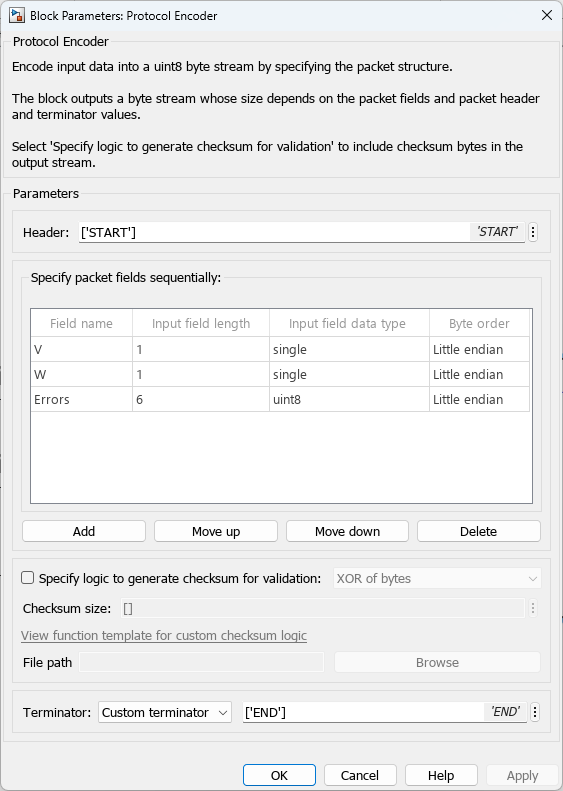
\includegraphics[width=1\textwidth]{imagenes/Simulink - Block Parameters - Protocol Encoder Arduino.png}
         \caption{Protocol Encoder}
     \end{subfigure}
     \hfill
     \begin{subfigure}[c]{0.45\textwidth}
         \centering
         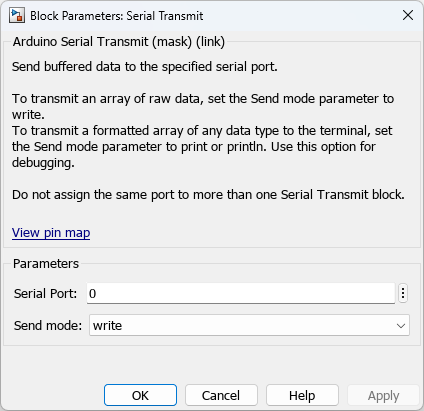
\includegraphics[width=1\textwidth]{imagenes/Simulink - Block Parameters - Serial Transmit Arduino.png}
         \caption{Serial Transmit}
     \end{subfigure}
        \caption{Parámetros de los bloques.}
\end{figure}

\subsection{Odometría}

Este subsistema calcula la posición y orientación del vehículo en función de sus velocidades lineal y angular y visualiza la trayectoria del vehículo en un plano \textit{XY}.

\begin{figure}[H]
    \centering
    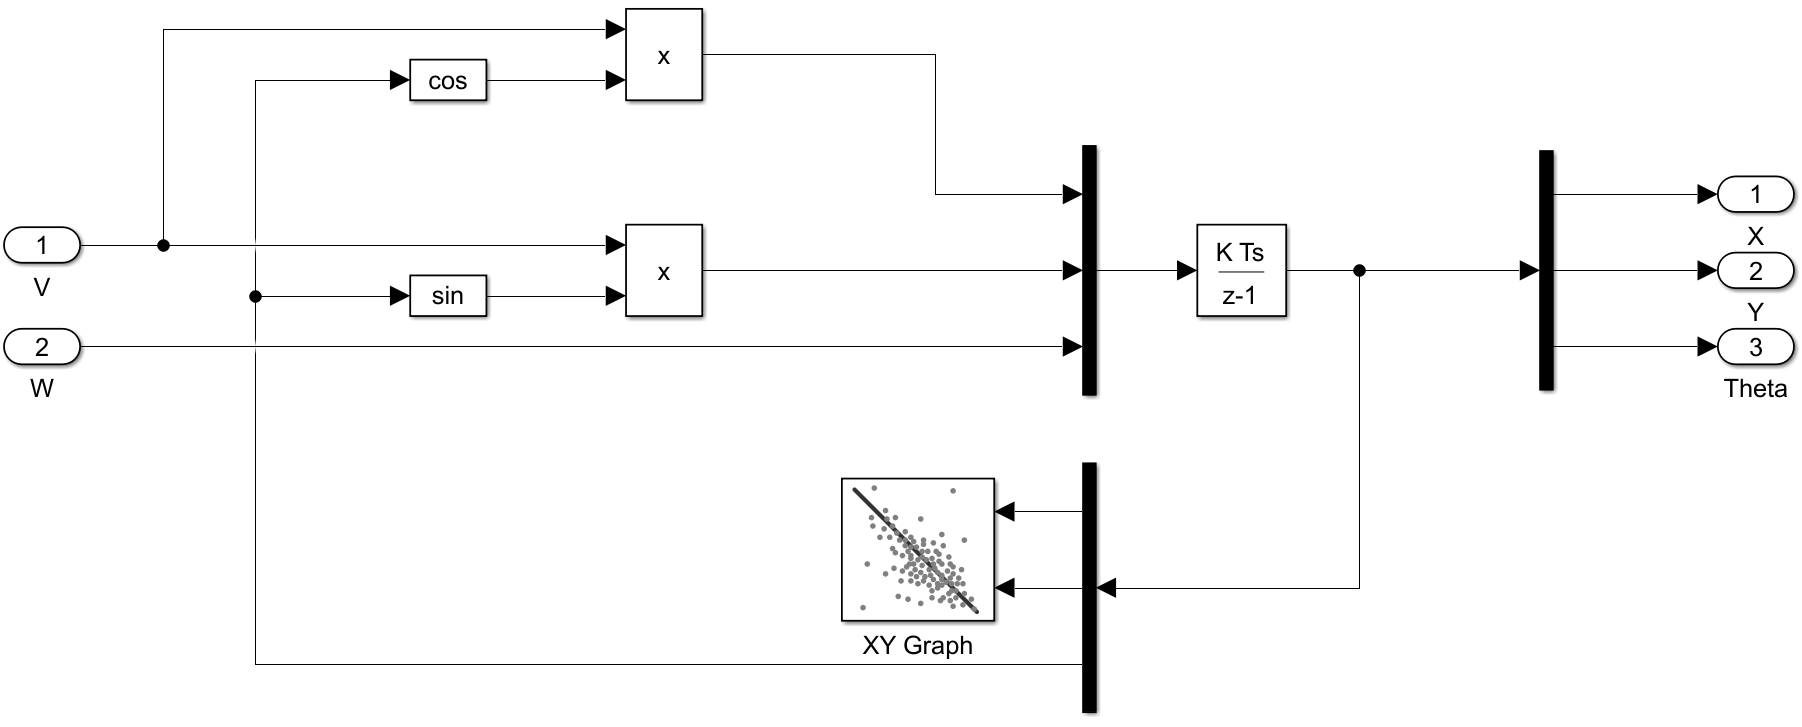
\includegraphics[width=1\linewidth]{imagenes/Simulink - Subsystem - Odometria.png}
    \caption{Subsistema Odometría}
    \label{fig:Subsistema - Odometria}
\end{figure}

Las ecuaciones que definen este sistema son:

\begin{equation}
    X = \int v_x dt= \int v \times cos(\theta) dt
\end{equation}

\begin{equation}
    Y = \int v_y dt = \int v \times sin(\theta) dt
\end{equation}

\begin{equation}
    \theta = \int \omega dt
\end{equation}

donde:

\begin{itemize}
    \item \(X\): Posición del vehículo en el eje X.
    \item \(Y\): Posición del vehículo en el eje Y.
    \item \(v_x\): Velocidad lineal en el eje X.
    \item \(v_y\): Velocidad lineal en el eje Y.
    \item \(\theta\): Ángulo de orientación del vehículo.
\end{itemize}

\section{Modelo control vehículo}

Los subsistemas descritos previamente serán los que integren este modelo. Su función será la de recibir la consigna de velocidad linear y angular desde el ordenador, transformar esta en velocidades específicas para cada motor, dependiendo de estas se establecen los demás parámetros de control de las ruedas y se transmiten. Partiendo de los motores se reciben las velocidades de cada uno que haciendo uso del modelo cinemático directo transformaremos en velocidad linear y angular del vehículo, transmitiendo finalmente esta información de nuevo al ordenador.

\begin{figure}[H]
    \centering
    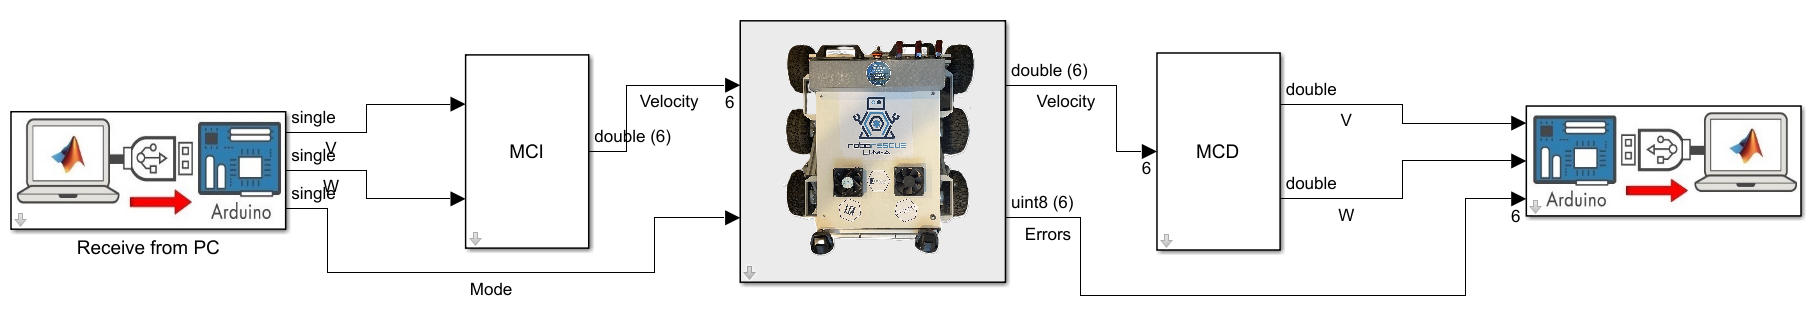
\includegraphics[width=1\linewidth]{imagenes/Simulink - Control Vehiculo.png}
    \caption{Modelo Control Vehículo}
\end{figure}

%\blankpage